\begin{figure}[t!]
	\vspace{-10px}
	\centering
	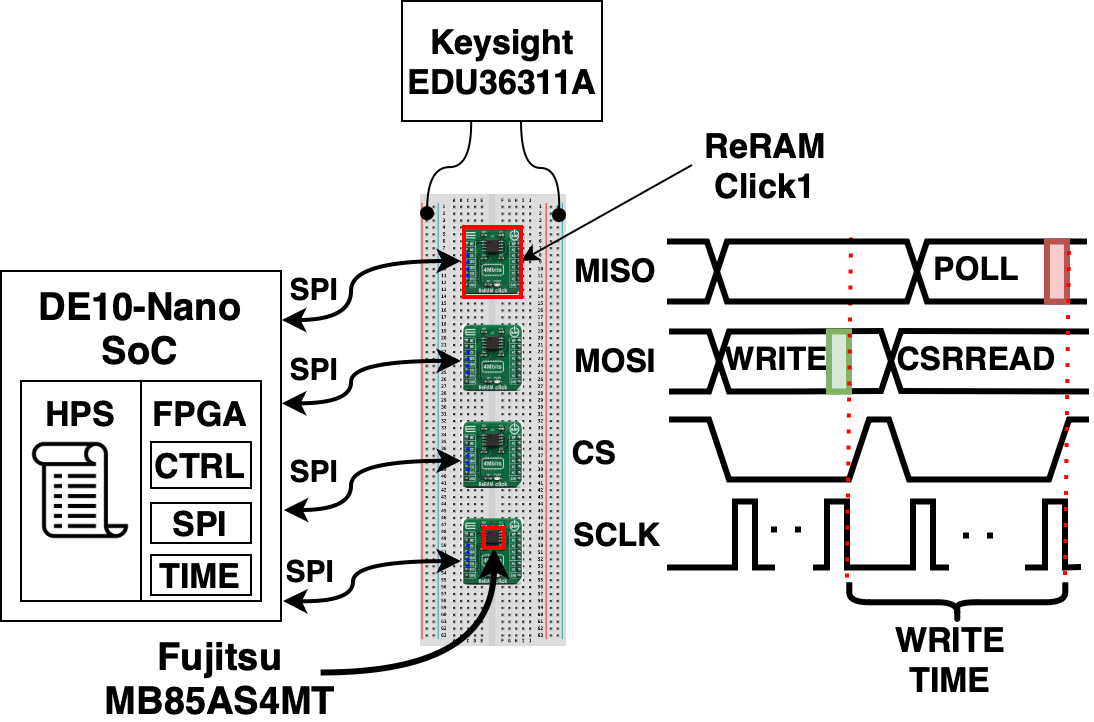
\includegraphics[width=0.75\linewidth]{img/experimental_setup.png}
	\caption{ReRAM memory instrumentation and WRITE transaction timing. An Altera DE10-Nano SoC FPGA system communicates to several Fujitsu MB85AS4MT (or MB85AS8MT) ReRAM memories via SPI. The ReRAM modules are connected to a separate EDU36311A DC power supply. The DE10-Nano is configured to measure the duration of SPI WRITE transactions \label{fig:expt-setup}.}
\end{figure}